\documentclass[12pt]{article}
\usepackage[utf8]{inputenc}
\usepackage[english]{babel}
\usepackage{amsmath}
\usepackage{amsfonts}
\usepackage{amssymb}
\usepackage{bbm}
\usepackage{tikz}
\usepackage{mathtools}
\usepackage{subfigure}
\usepackage[hang]{footmisc}

\setlength{\footnotemargin}{2.5mm}
\usetikzlibrary{shapes,automata,arrows}
\graphicspath{{images/}{../images/}}
\setcounter{tocdepth}{1}

\newcommand{\transpose}[1]{#1^{\mathsf{T}}}
\newcommand{\inverse}[1]{#1^{-1}}
\newcommand{\iterate}[2]{#1^{(#2)}}
\newcommand{\parens}[1]{ \left( #1 \right) }
\newcommand{\prob}{\mathbb{P}}
\newcommand{\dee}{\mathrm{d}}
\renewcommand{\thesubtable}{\Roman{subtable}}
\DeclareMathOperator{\rank}{rank}
\DeclareMathOperator{\Null}{null}
\DeclarePairedDelimiterX{\norm}[1]{\lVert}{\rVert}{#1}
\DeclarePairedDelimiter{\abs}{\lvert}{\rvert}

\title{Exploring PageRank}
\author{Nathanael Gentry}
\date{30 April 2019}

\begin{document}
\maketitle



\section{Motivation}
In 1998, two Stanford students -- Sergey Brin and Larry Page -- endavored to
bring order to the World Wide Web. Even in 1995, the public Internet
contained about 2.5 million pages \cite{TotalNumberWebsites}, but search
techniques relied upon classical strategies for collections much smaller and
less interconnected than the nascent Internet. The students’ graduate project,
then hosted at \texttt{google.stanford.edu}, did not rely on simple
heuristics like URL length or date of publication; their program used the link
structure of the Web itself to decide how relevant a page was to a user's query.
Brin and Page thus defined their problem as a problem of spectral ranking, or
eigencentrality. Spectral ranking provides a tractable definition of an entity's
relative \textit{importance} within a collection and thus gives an excellent
heuristic for its relevance in a search query. In this paper, we explore the
foundation of the Google enterprise: PageRank, the algorithm that provides a
spectral ranking of all pages on the indexed Web.



\section{First Steps}
\begin{figure}[h]
  \centering \scalebox{0.75}{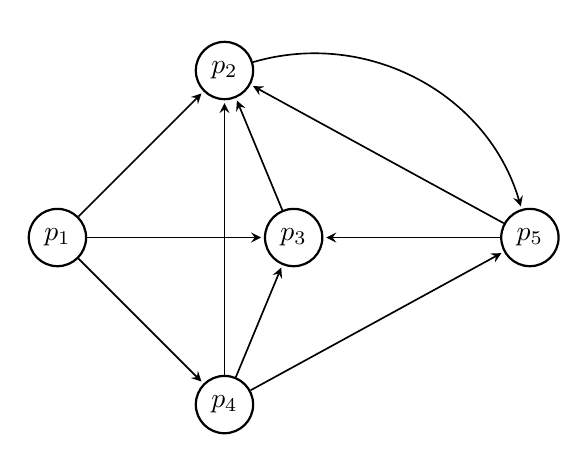
\begin{tikzpicture}[
			scale=0.6,
      > = stealth,
			shorten > = 1pt,
			auto,
			node distance = 3cm,
			semithick]
			\tikzstyle{every state}=[
			draw = black,
			thick,
			fill = white,
			minimum size = 4mm]

			\node[state] (a) {$p_1$};
			\node[state] (b) [above right of=a] {$p_2$};
			\node[state] (c) [right of=a] {$p_3$};
			\node[state] (d) [below right of=a] {$p_4$};
			\node[state] (e) [right of=c] {$p_5$};

			\path[->] (a) edge node {} (b);
			\path[->] (a) edge node {} (d);
			\path[->] (a) edge node {} (c);
			\path[->] (c) edge node {} (b);
			\path[->] (d) edge node {} (c);
			\path[->] (e) edge node {} (b);
			\path[->] (b) edge [bend left=45] node {} (e);
			\path[->] (d) edge node {} (b);
			\path[->] (e) edge node {} (c);
			\path[->] (d) edge node {} (e);
		\end{tikzpicture}}
  \caption{A Miniscule Web}
  \label{fig:web}
\end{figure}
Consider a digraph $\mathcal{W}$, such as that given in Figure \ref{fig:web}.
Each vertex $p$ represents a Web page, and each edge represents the existence of
at least one hyperlink between pages $p_i$ and $p_j$. We seek to calculate the
importance of a Web page, and we can view a hyperlink to that page as an
endorsement of importance from the linking page. The more such votes of support
a page has, the more important it probably is. The votes of importance imparted
by a Web page should be distributed evenly across the pages it endorses. Let us
now formalize this intuition. Let $N^-_i$ represent the set of $p_i$'s
predecessors, and let $N^+_i$ represent the set of $p_i$'s successors. Note that
$|N^+_i|$ gives the out-degree of $p_i$. We thus define the importance score
$\pi_i$ of a page $p_i$:
\begin{equation}\label{eqn:pi_i}
  \pi_i = \sum_{p_j\in N^-_i}{\frac{\pi_j}{|N^+_i|}}.
\end{equation}

Equation \eqref{eqn:pi_i} gives an impredicative definition of an importance
score.\footnote{Logicians disagree about the distinction between
  \textit{recursion} and \textit{impredicativity}. In this paper, we take
  recursion to be constructive -- that is, recursion builds a class by feeding
  the results of a generator into itself. Impredicativity, however, defines an
  impredicative object $X$ as an instantiation of a class which itself contains
  $X$. Equation \eqref{eqn:pi_i} thus gives an impredicative definition of
  $\pi_i$.} We store all the $\pi_i$ in a vector $\pi$, which we take henceforth
as a row vector.\footnote{Some authors denote row vectors by transposing a
  column vector every time, but we have found this notation wearying. In this
  paper the probability distribution $\pi$ will always be given by a row vector,
  without indication of transposition.} Take some initial score vector
$\iterate{\pi}{0}$, say a uniform distribution $\pi = [1/|\mathcal{W}|]$. Then,
we define an iterative calculation for an iterator $t\geq 1$ to refine the
initial distribution:

\begin{equation}
  \label{eqn:pi_t}
  \iterate{\pi}{t+1}_i = \sum_{p_j\in N^-_i}{\frac{\iterate{\pi}{t}_j}{|N^+_i|}}.
\end{equation}
We encode the system given by Equation \eqref{eqn:pi_i} over $\mathcal{W}$ in a hyperlink matrix:
\begin{equation*}
  H(\mathcal{W})_{ij}=\begin{cases}
    1/|N^+_i|, & \text{if } p_i \in N^-_j; \\
    0, & \text{otherwise}.
  \end{cases}
\end{equation*}

Thus, we have the following iterative calculation:
\begin{equation}
  \iterate{\pi}{k+1} = \iterate{\pi}{k} H.
\end{equation}
The hyperlink matrix gives an adjacency matrix of $\mathcal{W}$ modified to
ensure that each nonzero row provides a probability distribution. By
construction, $H$ is nonnegative; that is, $H_{ij}\geq 0$ for all components.
\begin{figure}[t!]
  \centering
  \begin{subfigure}
    \centering
    $\begin{bmatrix}
      0 & 1/3 & 1/3 & 1/3 & 0 \\
      0 & 0 & 0 & 0 & 1 \\
      0 & 1 & 0 & 0 & 0 \\
      0 & 1/3 & 1/3 & 0 & 1/3 \\
      0 & 1/2 & 1/2 & 0 & 0
    \end{bmatrix}$
    \caption{Hyperlink Matrix for Figure \ref{fig:web}}
    \label{fig:hyperlink}
  \end{subfigure}
  \vspace{2em}
  \begin{subfigure}
    \centering
    \begin{tabular}{|c||c|c|c|c|c|}
      \hline
      $k$ & $\pi_1$ & $\pi_2$ & $\pi_3$ & $\pi_4$ & $\pi_5$ \\
      \hline\hline
      0 & 0.2 & 0.2 & 0.2 & 0.2 & 0.2 \\
      1 & 0 & 0.433 & 0.233 & 0.067 & 0.267 \\
      2 & 0 & 0.389 & 0.156 & 0 & 0.456 \\
      3 & 0 & 0.383 & 0.228 & 0 & 0.390 \\
      4 & 0 & 0.422 & 0.194 & 0 & 0.383 \\
      \hline
    \end{tabular}
    \caption{Score Iteration for Figure \ref{fig:web}}
    \label{fig:example_calculation}
  \end{subfigure}
\end{figure}

Figures \ref{fig:hyperlink} and \ref{fig:example_calculation} show the
hyperlink matrix and some iterative calculations for the digraph given in
Figure \ref{fig:web}. We simply rank the pages by the distribution given in
$\pi$.

Observe that $p_2$ has the highest rank, as most other pages point into it
and it only links to one page. However, this page $p_5$ also receives a high
score, since an important page directly links to it. Our na{\"i}ve approach
shuts out $p_1$ and $p_4$ entirely, which destroys the uniqueness of the
ranking. There are other problems with our formulation. Note that the zero
rows of $H$ correspond to dangling pages, i.e. vertices with zero
out-degree. These rank sinks will break our current calculation, but we
cannot simply exclude them. Some sinks -- for instance, published PDF
documents -- might be highly cited and quite important. Consider also the
trouble posed by cyclic graphs, which would eternally shift their importance
around their cycles. If we continued the iterative calculation in Figure
\ref{fig:example_calculation}, we would find the scores of $p_2$ and $p_5$
keep oscillating as the number of iterations grew. We will discuss the
problem of cyclicity later, but we easily fix can rank sinks by making $H$
fully row-stochastic.



\section{Markov Chains}


\subsection{Stochasticity}
Consider a vector $d$, where $d_i=1$ if page $p_i$ dangles and $d_i=0$
otherwise. Let $v$ be a distribution over all pages in a Web graph
$\mathcal{W}$. We stochasticize $H$ thusly:
\begin{equation}
  \label{eqn:S}
  S=H + d\transpose{v}.
\end{equation}

If an ideal ``random surfer'' on the Web hits a dangling page, it chooses based
upon the distribution $v$ what page to next visit. Let $\mathbbm{1}$ represent a
vector of ones, and note that the row-stochasticity of $S$ implies
$\Vert S \Vert_{\infty} = 1$, i.e. $S \mathbbm{1} = \mathbbm{1}$. Thus,
$(1, \mathbbm{1})$ provides a right eigenpair for every stochastic matrix. Now
consider an eigenpair $(v, \lambda)$ of a stochastic matrix $S$ and suppose
$|\lambda| > 1$. Then, the vector given by $|\lambda|^n v = S^n v$ grows
exponentially, so at least one $(S^n)_{ij} > 1$ for some $n$. This, however,
contradicts the stochasticity of $S$. Thus, we conclude that $|\lambda| \leq 1$,
and since we have already 1 as an eigenvalue, we conclude the spectral radius
$\rho(S)=1$. This result can be proved directly from the Gershgorin circle
theorem, but we will not explore that here.


\subsection{Transition Probability}
As noted above, we can view $S_{ij}$ as the probability that a random surfer on
a Web jumps from page $p_i$ to page $p_j$ at a given time. Thus, we can model
our spectral ranking problem as a Markov chain. In this conversation, we
consider homogeneous Markov chains -- those that have transition probabilities
independent of time. This probabalistic insight leads us to view $S$ as the
1-transition matrix of a finite-state, discrete-time Markov chain. Recall that a
discrete-time stochastic process $\{X_t\}_{t \in T}$ for a countable set $T$
over a finite $n$-sized state space $\Omega = \{s_i\}_{i\leq n}$ is a Markov chain if, for
each $t$, the Markov property holds. Markov chains are colloquially described by
\textit{memorylessness}, which the Markov property formalizes:
\begin{equation*}
  \prob(X_{t+1} = s_j \mid X_t = s_{i_t}, X_{t-1} = s_{i_{t-1}},\cdots, X_0 =
s_{i_0}) = \prob(X_{t+1} = s_j \mid X_t=s_{i_{t}}).
\end{equation*}
We encode the $k$-step transition probabilities for a homogeneous Markov chain
in a stochastic matrix of dimension $|\Omega| \times |\Omega|$:
\begin{equation}
  \iterate{P}{k} = [ \iterate{p}{k}_{ij} ] = [ \prob(X_{t+k} = s_j \mid X_t =
s_i) ] = [ \prob(X_{t} = s_j \mid X_0 = s_i) ].
\end{equation}
Note how the memorylessness of the Markov chain enables the powerful final
equality above. By the definition of the transition matrix, we see
$ [ \iterate{p}{1}_{ij} ] = P$. Now, suppose inductively that
$\iterate{p}{\ell}_{ij} = \parens{\iterate{P}{\ell}}_{ij}$ for all
$i, j \in \Omega$. Then, observe the following:
\begin{align*}
  \iterate{p}{1+\ell}_{ij} &= \prob(X_{\ell+1} = s_j \mid X_0 = s_i) \\
                           &= \sum_{s_k\in\Omega}{\prob(X_1 = s_k \mid X_0 = s_i) \prob(X_{1+\ell} = s_j \mid
                             X_1 = s_k)} && \text{(total probability)} \\
                           &= \sum_{s_k\in\Omega}{\prob(X_1 = s_k \mid X_0 = s_i) \prob(X_{\ell} = s_j \mid X_0 = s_k)} &&
                                                                                                                           \text{(homogeneity)} \\
                           &= \sum_{k\leq
                             |\Omega|}{\parens{\iterate{p}{1}_{ik}\iterate{p}{\ell}_{kj}}}
                           && \text{(definition of transition matrix)}\\
                           &= p^{1+\ell}_{ij}. && \text{(matrix multiplication)}
\end{align*}
From this result, we derive the Chapman-Kolmogorov equations:
\begin{equation}
  \iterate{p}{m+n}_{ij} = \sum_{k\leq |\Omega|}{\parens{\iterate{p}{n}_{ik} \iterate{p}{m}_{kj}}}
\end{equation}

We will denote the $k$-step transition probability from state $s_i$ to $s_j$ by
directly referencing the components of the transition matrix. Since Markov
chains are memoryless, we simply take each successive iteration as if it were
the first; in this way, we understand that iteration of transitions is given by
matrix multiplication in a homogenous chain. Recall that $k$-paths of graphs are
also given by the $k^\text{th}$ power of the adjacency matrix.

With this in mind, consider a distribution $\iterate{v}{\ell}$ over $\Omega$,
defined by $\iterate{v}{\ell}_i = \prob(X_\ell = i)$. Then, by the total law of
probability, we calculate the following:
\begin{align*}
  \iterate{v}{\ell}_i &= \sum_{s_k\in\Omega}{\prob(X_0 = s_k) \prob(x_\ell = s_i \mid X_0 = s_k)} \\
                      &= \sum_{k\leq |\Omega|}{\parens{\iterate{v}{0}_k \iterate{p}{\ell}_{ki}}}.
\end{align*}

From these results, we conclude that
$\iterate{v}{\ell} = \iterate{v}{0} \iterate{P}{\ell} = \iterate{v}{0} P^\ell$,
for some initial iterate $\iterate{v}{0}$. We have now more clearly justified
the construction of equation \eqref{eqn:pi_t}.


\subsection{Stationarity}
We may take the stochastic process $\{X_t\}_{t \in T}$ underlying a Markov chain
as a categorical distribution over $\mathcal{S}$, the state space.\footnote{The
  categorical (multinoulli) distribution is a generalization of the Bernoulli
  distribution, where each random variable may take one of $k$ states.} A chain
distribution $\pi$ gives a simplex of dimension $|S| - 1$. Choose such a
$P$-invariant simplex. By Brouwer's fixed point theorem, within this simplex
must be a $P$-invariant distribution, i.e., a
$P$-eigenvector.\footnote{Brower's fixed point theorem leads to an elegeant
  argument for Perron's theorem of positive matrices. Michael Brin -- Sergey's
  father -- first advanced such topological arguments for Perron-Frobenius
  theory in 1993. We encourage the reader to consult
  \cite{boyleBasicPerronFrobeniusTheory} for more details. \vspace{0.5em} \\
  Note further that the simplexical argument for the stationary distribution is
  interesting but not at all constructive. We can, in fact, construct an exact
  definition of $\pi$ from the expected number of visits to each state in a
  positive recurrent chain. See \cite{freedmanConvergenceTheoremFinite} for an
  excellent summary of these probabalistic arguments. In this paper, we take a
  linear-algebraic approach to convergence via the Perron-Frobenius theorem. In
  hindsight, we see that our route of exposition might have been the messier
  option. However, since Google determines PageRank through power iteration on
  the transition matrix, our conversation shows more clearly how PageRank works
  in the real world.} We denote this fixed distribution $\pi$ such that
$\pi P = \pi$. That is, $\pi_i = \prob(X_t = s_i)$ for all $t\in T$ over all
states. This time independence defines the stationarity of a distribution $\pi$,
and it thus gives an eigenequation for spectral analysis. Consider a stationary
distribution $\pi$ that is also a limiting distribution, so that we have the
following:
\begin{equation*}
  \pi = \lim_{k\to\infty}{{\iterate{\pi}{k}}} = \lim_{k\to\infty}{\parens{{\iterate{\pi}{0}} P^k}}.
\end{equation*}

In a Markov chain with a limiting distribution, any initial distribution
$\iterate{\pi}{0}$ will eventually converge upon $\pi$. However, a stationary
distribution does not itself imply a limiting distribution. For instance,
consider the Markov chain given by
$P=\begin{bsmallmatrix} 0 & 1 \\ 1 & 0 \end{bsmallmatrix}$. This standard
example corresponds to turning a coin over, so the opposite state is reached
with certainty at each step. However, the probability of revealing a certain
face at a given step depends entirely upon the initial state -- what face of the
coin was initially facing up. Thus, this chain does not have a limiting
distribution. However, we have an easy stationary distribution:
$v = [\frac{1}{2}, \frac{1}{2}]$, corresponding to choosing the initial state by
flipping a fair coin. The stationary distribution hides the chain's dependence
upon its initial state. However, if we have a biased coin, say one for which
$\iterate{v}{0} = [\frac{3}{5}, \frac{4}{5}]$, the transition probabilities at
each turn of the coin clearly depend upon the initial state of the coin.

We can also show that no limiting distribution exists by examining the
transition matrix. As $k\to\infty$, the iterate $\iterate{P}{k}$ swaps certainty
of transition between states; it alternates between $P$ and $I$. Thus, the limit
of the transition matrix does not exist, and so a limiting distribution does not
exist.

The nature of our spectral ranking problem thus becomes stunningly clear, for
the time-independent probabilities within $\pi$ yield a unique metric of the
importance we have sought to codify. We can predict, from the structure of the
Web itself, how much time a random Web surfer will spend on a given page, and we
can take these probabilities as evidence for how important a page actually is.
Analyzing the asymptopic behavior of $P$ will show us when such a limiting
distribution exists, and we will thus know when we have a unique solution to the
stationary eigenequation. We now answer the vital question of when a Markov
chain has such distribution by exploring a fundamental theory of dynamical
systems.




\section{Perron-Frobenius Theory}


\subsection{Irreducibility}
In a Markov chain, states $s_i$ and $s_j$ communicate if
$\iterate{P}{k}_{ij} > 0$, for some iterate $k$. That is, there is a path of
nonzero probability (a random walk) between states $s_i$ and $s_j$.
Communicativity is easily shown to be an equivalence relation.

Consider partitioning a Markov state space $\Omega$ of size $n$ into partitions
$\Omega_1 = \{ s_i \}_{i\leq k}$ and $\Omega_2 = \{ s_j \}_{k < j \leq n}$.
Moreover, suppose there are random walks from $\Omega_2$ to $\Omega_1$ but none
the other way. Note that the chain eventually never visits states in $\Omega_2$;
when $\Omega_1$ is a communicating class, the chain reduces to the states of
$\Omega_1$. We model such reducibility of a Markov chain in a lower-triangular
canonical form:
\begin{equation*}
  \label{eqn:reducible}
  P =
  \begin{bmatrix}
    \omega_{1\to 1} & 0 \\
    \omega_{2 \to 1} & \omega_{2 \to 2}
  \end{bmatrix},
\end{equation*}
where $\omega_{1\to 1}$ and $\omega_{2\to 2}$ are substochastic square matrices
representing transition probabilities within $\Omega_1$ and $\Omega_2$,
respectively, and $\omega_{2 \to 1}$ holds the transition probabilities from
$\Omega_2$ to $\Omega_1$. Note that when $\omega_{2\to 1} = 0$, the chain is
disconnected and so \textit{completely} reducible.

We say a Markov chain is irreducible if and only if it contains a single
communicating class. Equivalently, a digraph is irreducible when it has no
strongly connected components (SCCs) smaller than itself.\footnote{Note that a
  topological sort on a reducible graph can factorize it into its disjoint
  strongly-connected components.} An irreducible matrix is a matrix
corresponding to such irreducible objects. Note that an irreducible matrix is
nonnegative; the transition matrix motivation above shows the classes of
reducibility and irreducibility arise through the arrangement of zeroes within
the matrix. To find reducbility in a chain-graph, we simply attempt to permute
the state-vertices in the underlying matrix to obtain the above canonical form.

Consider further what reducibility means in a Markov chain. As time passes, the
probability of visiting the pages in $\Omega_2$ drops to zero. To our iterative
importance calculation on Web pages, these pages will eventually appear not at
all important, but there is no reason why they shouldn't be. We must not permit
this artifact of the Web structure to corrupt our importance scores. For now, we
take reducibility of a Markov chain as a hypothetical difficulty; later, we will
see that the real Web is quite reducible and requires a less naïve model to give
convergent and unique importance scores.


\subsection{Periodicity}
Consider a Markov chain with states $s_i \in \mathcal{S}$. Let
$D(s_i) = \{n\in \mathbb{Z}_{\geq 0} : \iterate{p}{n}_{ii} > 0 \} \subset
\mathbb{N}$. Note that $D(s_i)$ is trivially nonempty, as
$\iterate{p}{0}_{ii} = 1$ for all $s_i$. We observe that $D(s_i)$ forms a
numerical semigroup under addition. We define the period of a state by
$d(s_i)=\text{gcd}\{D(s_i)\}$. In other words, a random walk (a path where each
step has nonzero probability) from state $s_i$ can only return to $s_i$ in
multiples of $d(s_i)$ steps. Consider states $s_i$ and $s_j$ in the same
communicating class. Thus, $\iterate{p}{m}_{ij} > 0$ and
$\iterate{p}{n}_{ji} > 0$ for some nonnegative iterators. Otherwise stated,
consider a random $m$-path from $s_i$ to $s_j$ and a a random $n$-path from
$s_j$ to $s_i$.
\begin{figure}[h]
  \centering \scalebox{0.75}{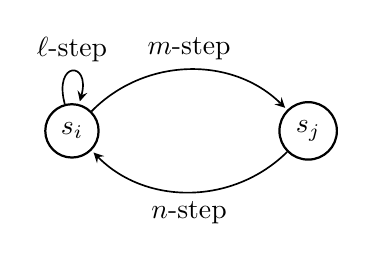
\begin{tikzpicture}[
			scale=0.6,
      > = stealth,
			shorten > = 1pt,
			auto,
			node distance = 3cm,
			semithick]

			\tikzstyle{every state}=[
			draw = black,
			thick,
			fill = white,
			minimum size = 4mm]

			\node[state] (a) {$s_i$};
			\node[state] (b) [right of=a] {$s_j$};

			\path[->] (a) edge [bend left=45] node {$m$-step} (b)
      (a) edge [loop above]   node {$\ell$-step} (a)
      (b) edge [bend left=45] node {$n$-step} (a);
		\end{tikzpicture}}
  \caption{Communicating States}
  \label{fig:markov}
\end{figure}

Figure \ref{fig:markov} illustrates these cycles. Note that there are random
cycles of length $\ell \equiv m+n \pmod{d(s_i)}$ on state $s_i$. The
communicativity of $s_i$ and $s_j$ implies $\iterate{p}{n+m}_{jj} > 0$ and
$\iterate{p}{n + \ell + m}_{jj} > 0$. That is, there is a random $\ell$-cycle on
$s_j$; moreover, there is a random cycle on $s_j$ that goes from $s_j$ to $s_i$
and returns to $s_i$ before terminating at $s_j$. Thus, $d(s_j) \mid \ell$.
However, since we have shown that $s_i$ has a random $\ell$-cycle, we know that
$d(s_j) \mid d(s_i)$. By the symmetry of $s_i$ and $s_j$, we find
$d(s_i) \mid d(s_j)$, and so $d(s_i) = d(s_j)$ whenever $s_i$ and $s_j$
communicate. Thus, when $P$ is irreducible, $d(P)$ is well-defined; every state
has the same period. When $d(P) = 1$, we say the Markov chain is aperiodic.


\subsection{Primitivity}
Much has been said on the conditional convergence of periodic Markov chains, but
we confine this conversation to the aperiodic case. Suppose we have an aperiodic
irreducible Markov chain, and recall $D(s_i)$, the numerical semigroup given
above.\footnote{Markovian semigroups form an important part of ergodic theory,
  which we barely explore here.} For a semigroup $V$ with $d=\gcd(V)$, it can be
shown that there exists an integer $N$ such that $v\equiv n \pmod{d}$ for any
$v\in V$ and all $n \geq N$. Since we have supposed an aperiodic Markov chain,
we have a coprime numerical semigroup. Thus, there is some bound $t_i$ beyond
which $\iterate{p}{t}_{ii} > 0$ for all $t \geq t_i$ over all states. By the
irreducibility of the chain, we have a $k = k_{(i,j)}$ for which
$\iterate{p}{k}_{ij} > 0$. Thus, for $t \geq t_i + k$, the Chapman-Kolmogorov
equations yield the following:
\begin{align*}
  \iterate{p}{t}_{ij} \geq \iterate{p}{t-k}_{ii} \iterate{P}{k}_{ij} > 0.
\end{align*}
Let $t'_i = t_i + \max_{j\in\Omega}\{ k_{(i,j)} \}$. Thus, for $t \geq t'_i$, we
have $\iterate{p}{t}_{xy} > 0$ for all $y\in\Omega$. Then, for
$t \geq \max_{i\in\Omega}\{ t'_i \}$, we conclude that, for an irreducible
aperiodic chain, there is a $t$ that gives $\iterate{p}{t}_{ij} > 0$ over all
states, and so $P^t > 0$. We take this result as the definition of matrix
primitivity.

Primitivity is irreducibility plus aperiodicity. Recall that a merely
irreducible Markov chain requires an iterate-function of state pairs. However, a
primitive chain guarantees that \textit{all} states communicate -- not just that
they are a part of the same communicating class -- after $t$ transitions.

Consider a primitive Markov chain with eigenpair $(v, \lambda)$. The underlying
primitivity of the transition matrix $P$ gives $P^k v = \lambda^k v > 0$ for
some iterate $k$ and forever thereafter, so we see the eigenpair must be
positive. Take another eigenpair $(w, \gamma)$ such that $\norm{w} < \norm{v}$
and $\gamma = \rho(P)$. Then for all iterates $n$, we have the following:
\begin{equation*}
  \gamma^n w = P^n w \leq P^n v = \lambda^n v.
\end{equation*}
However, since we supposed $\norm{w} < \norm{v}$, we cannot have
$\beta < \lambda$. By the inequality above, we must conclude $\beta = \lambda$,
and so a primitive $P$ has only one eigenvalue on its spectral circle, namely
the spectral radius itself. This eigenvalue is the dominant eigenvalue of $P$.
Since all stochastic matrices have spectral radius 1, we conclude that primitive
Markov chains have an eigenpair $(1, \pi)$. This is exactly what we want to
satisfy our limiting distribution condition $\pi = \pi P$. The following
spectral properties of primitive Markov chains should not be terribly surprising
by now, but they are are quite beautiful.


\subsection{Perron-Frobenius Theorem}
Perron's theorem, proved in 1907, provided spectral properties of positive
matrices -- most notably, that such matrices have only one eigenvalue on their
spectral circle, the dominant eigenvalue $\lambda_1=\rho(A)$. However, Perron's
results results did not generally apply to nonnegative matrices. Frobenius
subsequently realized that irreducible matrices behave like positive matrices,
except that they may have multiple eigenvalues that are roots of unity of
$d(P)$. Primitive matrices, however, do have a dominant eigenvalue, as we have
seen above. The Perron-Frobenius theorem, proved in 1912, gives the following
properties for a primitive square matrix:
\begin{enumerate}
\item The spectral radius $\rho$ equals some real eigenvalue $\lambda_1$;
\item This eigenvalue (the Perron root) is simple, and it is the only eigenvalue on the spectral circle;
\item The Perron root has unique, strictly positive left and right eigenvectors (Perron vectors);
\item These left and right Perron eigenvectors are, up to normalization, the only nonnegative eigenvectors of $A$.
\end{enumerate}
Note that the Perron root is a dominant eigenvalue; it is the unique $\lambda_1$
such that $|\lambda_1|>|\lambda_2|\geq\cdots\geq |\lambda_{n}|$ for all
$\lambda \in \sigma(A)$. Recall that $A$ and $\transpose{A}$ share a spectrum,
and a left eigenvector of $A$ is a right eigenvector of $\transpose{A}$.

We will not prove the complete Perron-Frobenius theorem in this paper -- its
full statement contains far more than we have given here -- although we have
heretofore outlined some basic arguments for the properties we find useful for
spectral ranking.




\section{Limiting Distributions}


\subsection{Spectral Resolution\protect\footnote{The results in this section
    summarize the extended treatment of matrix functions and convergence given
    in \cite{meyerMatrixAnalysisApplied2000}}.}
Recall that, for a a diagonalizable matrix $A=PD\inverse{P}$, the columns of the
similarity transformation $P$ correspond to distinct right eigenvectors of $A$.
Consider partitioning $P$ into bases $\beta_{\mathcal{E}_\lambda}$ for distinct
right eigenspaces of $A$. Similarly, we partition the rows of $\inverse{P}$ into
bases $\gamma_{\mathcal{E}_\lambda}$ for distinct left eigenspaces. Thus, for a
matrix $A$ with with spectrum $\sigma$, we have an outer product formulation of
the spectral decomposition:
\begin{equation}
  \label{eqn:spectral_decomposition}
  A = PD\inverse{P} = \sum_{\lambda\in\sigma}{\lambda [\beta_{\mathcal{E}_\lambda}]\transpose{[\gamma_{\mathcal{E}_\lambda}]}}.
\end{equation}

Note that
$E_\lambda =
[\beta_{\mathcal{E}_\lambda}]\transpose{[\gamma_{\mathcal{E}_\lambda}]}$
projects onto the eigenspace $\mathcal{E}_\lambda$. In fact, $A$ is
diagonalizable if and only if it can be written as a sum of such spectral
projectors. Consider $x$ and $\transpose{y}$ as the handed eigenvectors of a
simple eigenvalue $\lambda_s$. We see this elegant formula for the corresponding
eigenprojection:
\begin{equation}
  \label{eqn:simple_eigenprojection}
  E_{\lambda_s} = \frac{x \transpose{y}}{\transpose{y} x},
\end{equation}
where the inner product in the denominator comes from normalization to ensure projection properties.


\subsection{Matrix Functions}
Consider generalizing a scalar function $f$ to be a matrix function. As the
well-known matrix exponential illustrates, we often do not define matrix
functions as scalar functions applied entrywise, for we then might lose the nice
properties associated with the scalar functions. Using the Taylor expansion of a
sufficiently-differentiable $f$, we first define such a function about a Jordan
block $J_k(\lambda)$:
\begin{equation*}
  f\big( J_k(\lambda) \big)=f(\lambda)I + f'(\lambda)(J_k(\lambda) - \lambda I) + \frac{f'(\lambda)(J_k(\lambda) - \lambda I)^2}{2!} + \cdots.
\end{equation*}
However, since $(J_k(\lambda) - \lambda I)$ is nilpotent of order $k$, the
Taylor expansion reduces nicely:
\begin{equation}
  \label{eqn:f_jordan_block}
  f\big( J_k(\lambda) \big) = \sum_{i=0}^{k - 1}\parens{\frac{f^{[i]}(\lambda)}{i!} (J_k(\lambda) - \lambda I)^i}.
\end{equation}

Thus, for $f$ with at least $(k - 1)$ derivatives that exist at $\lambda$, we
have the definition of a function applied to a Jordan block:
\begin{equation}\label{eq:f_jordan_block}
  f\big( J_k(\lambda) \big) =
  \begin{bmatrix}
    f(\lambda) & f'(\lambda) & \frac{f''(\lambda)}{2!} & \ldots & \frac{f^{[k - 1]}(\lambda)}{(k-1)!} \\
    0 & f(\lambda) & f'(\lambda) & \ldots & \frac{f^{[k - 2]}(\lambda)}{(k-2)!} \\
    0 & \vdots & \vdots & \ddots & \vdots \\
    0 & 0 & 0 & \ldots & f(\lambda)
  \end{bmatrix}.
\end{equation}

For a diagonalizable matrix $A$ as above, note that we can we apply Equation
\eqref{eqn:spectral_decomposition} to obtain a nice result:
\begin{align*}
  f(A) = Pf(D)\inverse{P} = \sum_{\lambda \in \sigma}{f(\lambda) E_\lambda}.
\end{align*}

We can extend $f$ to a Jordan form $J$ by requiring that $f$ has at least
$(\iota - 1)$ derivatives, where $\iota = \iota_\lambda$ is the index of
$\lambda$, i.e., the size of the largest $\lambda$-block. Then, for $A$ with
spectrum $\sigma$, not necessarily diagonalizable, we have this function
definition:
\begin{equation*}
  f(A) = P f(J) \inverse{P} = \sum_{\lambda \in \sigma}\parens{ [\beta_{\mathcal{E}_\lambda}]\, f\big( J_{k_\lambda}(\lambda) \big)\, \transpose{[\gamma_{\mathcal{E}_\lambda}]} }.
\end{equation*}
Expanding the definition of the function and applying the eigenprojection gives
this form:
\begin{equation}
  f(A) = \sum_{\lambda \in \sigma}\sum_{j=0}^{\iota_{\lambda} - 1}\parens{ \frac{f^{[j]}(\lambda)}{i!} (J_{k_\lambda}(\lambda) - \lambda I)^j E_{\lambda} }.
\end{equation}


\subsection{Matrix Convergence}
Consider the function $f(x) = x^n$ for some real $n$. Note that when we apply
$f$ to a Jordan block, we can easily give the coefficients of differentiation as
binomial coefficients.
\begin{equation}\label{eq:power_jordan_block}
  \big( J_k(\lambda) \big)^n =
  \begin{bmatrix}
    \lambda^n & \binom{n}{1}(\lambda^{n-1}) & \binom{n}{2}(\lambda^{n-2}) & \ldots & \binom{n}{k-1}(\lambda^{n-(k+1)}) \\
    0 & \lambda^n & \binom{n}{1}(\lambda^{m-1}) & \ldots & \binom{n}{k-2}(\lambda^{m-(k+2)}) \\
    0 & \vdots & \vdots & \ddots & \vdots \\
    0 & 0 & 0 & \ldots & \lambda^n
  \end{bmatrix}.
\end{equation}
In general, then, we define $f(A)$ thusly:
\begin{equation}
  A^n = \sum_{\lambda \in \sigma}\sum_{j=0}^{\iota_{\lambda} - 1}\parens{ \binom{n}{j} \lambda^{n-j} (J_{k_\lambda}(\lambda) - \lambda I)^j E_{\lambda} }.
\end{equation}

Suppose $| \lambda | < 1$. Then, for each $j \in [1, n-(k+1)]$, we have
\begin{equation*}
  \abs*{\binom{n}{j}\lambda^{m-j}} \leq \frac{k^j}{j!}{\abs*{\lambda^{m-j}}}.
\end{equation*}
Note that as $m \to \infty$, the numerator $k^j$ diverges polynomially since $j$
is fixed. However, since $| \lambda | < 1$, $\abs{\lambda^{m-j}}$ converges to
zero exponentially. Thus, we conclude the following:
\begin{equation*}
  \lim_{n\to\infty}{\big( J_k(\lambda) \big)^n} = 0.
\end{equation*}
We can extend this argument to show that, for a square matrix $A$,
$\lim_{n\to\infty}{\parens{A^n}} = 0$ if and only if $\rho(A) < 1$, and similar
reasoning shows the limit does not exist when $\rho(A) > 1$.

We now study the convergence of a matrix with $\rho(A) = 1$, such as we have
with all stochastic (and primitive) matrices. Suppose we have a primitive Markov
chain with transition matrix $P$. By the Perron-Frobenius theorem, we know $P$
has dominant eigenvalue $\lambda_1 = 1$. As all non-dominant eigenvalues have
modulus less than 1, we simply have the following:
\begin{equation*}
  \lim_{n\to\infty}{A^n} = E_{\lambda_1}.
\end{equation*}
Powers of a primitive matrix will eventually converge upon the dominant
eigenprojector. For primitive Markov chains, we have a left eigenvector $\pi$,
the stationary distribution. Moreover, we previously showed that all stochastic
matrices have right eigenvector $\mathbbm{1}$. Thus, using the limit we just
discovered, we have a limiting distribution:
\begin{equation}
  \lim_{k\to\infty}{{\iterate{\pi}{k}}} = \lim_{k\to\infty}{\parens{{\iterate{\pi}{0}} P^k}} = \iterate{\pi}{0} \parens{\frac{\mathbbm{1} \pi}{\pi \mathbbm{1}}} = \parens{\iterate{\pi}{0} \mathbbm{1}} \pi = \pi.
\end{equation}
Thus, primitivity guarantees a distribution completely independent of the
chain's starting state. The convergence of a primitive chain is a rather
remarkable result, one often called the fundamental theorem of Markov chains.


\subsection{Power Iteration}
Applying Perron-Frobenius theory to primitive Markov chains gives a classical
method for calculating the limiting distribution. Techniques based on Gaussian
elimination would not be a smart choice for calculating a limiting distribution
$\pi$ of the Internet, since this family of alogrithms generally has arithmetic
complexity of order $O(n^3)$.

Here, we explore the power method -- the simplest iterative calculation method.
Suppose a square matrix $A$ has $n$ eigenpairs $\{ (\lambda_i,x_i) \}_{i\leq n}$
with $\lambda_1$ as a dominant eigenvalue. Consider a starting vector
$x^{(0)}=\sum_i{\gamma_i x_i}$ for scalars $\gamma_i$. Then, we again consider
an iterative calculation:
\begin{equation}
  \iterate{x}{k} = A^k \iterate{x}{0} = \sum_{i=1}^{k}{\gamma_i \lambda_i^k x_i} = \lambda_1^k\parens{\gamma_1 x_1 + \sum_{i=2}^{k}{\gamma_i \frac{\lambda_i}{\lambda_1} x_i}} \to \lambda_1^k \gamma_1 x_1.
\end{equation}
Since $\lambda_i<\lambda_1$ for $i>1$, the sum approaches 0 as $k\to\infty$. The
speed of convergence clearly depends upon the subdominant eigenvalue
$\lambda_2$. Power method applications often normalize the the estimated
eigenvector after each iteration to avoid underflow or overflow under successive
powers of the eigenvalue, but we need not worry about this since primitive
Markov chains have dominant eigenvalue $\lambda_1 = 1$.



\section{The Google Matrix}
Deriving a limiting distribution from the Web graph still requires a bit more
work, for the real Web is quite reducible.
\begin{figure}
  \centering
  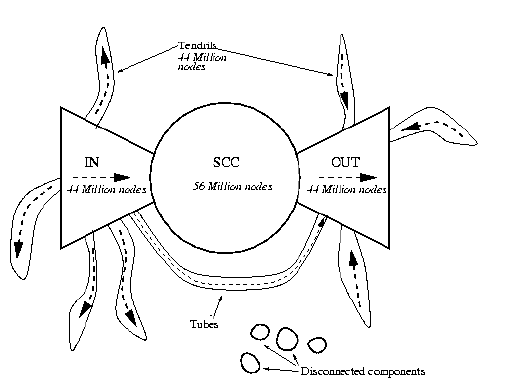
\includegraphics[scale=0.6]{bow-tie}
  \caption{The Bow Tie \cite{broderGraphStructureWeb}}
  \label{fig:bow-tie}
\end{figure}
In 1999, \cite{broderGraphStructureWeb} crawled over 1.5 billion links to
generate a comprehensive map of the Web. Their macroscopic figure, given in
Figure \ref{fig:bow-tie}, stylizes the Web super-graph as a rather eldritch bow
tie. Note that the figure has the form of a directed acyclic graph given from a
topological sort. In the middle is the ``bow knot'' -- the largest
strongly-connected component (SCC) of the Web. In 2012, when the last public Web
mapping occured, about half of mapped Web pages were strongly connected. The
``thistle ends'' of the tie, denoted \texttt{IN} and \texttt{OUT}, respectively
reference pages from which surfers can link into (out of) the SCC but cannot
return by the same route. Pages within the tendrils and tubes are likewise
unidirectional on this macroscopic scale: They be reached from \texttt{IN} and
\texttt{OUT}, but these components cannot be reached from within them. Although
the numbers in Figure \ref{fig:bow-tie} are obsolete, its bow-tie model wtill
describes the Web well.

We previously eliminated individual dangling pages, but we could view these
entire tendrils and tubes again as ``dangling pages,'' and we can again correct
for them. In our Markov discussion, we interpreted the stochastic Web matrix $S$
as the matrix of probabilities that an ideal random surfer follows links from a
page or chooses another randomly when it hits a dead end. However,
\textit{human} Web surfers often get bored. They will not follow a linear path
through the Web; they might suddenly elect to teleport -- shift course
altogether and visit a page on whim. Let $\mathbbm{1}$ represent a vector of
ones, and again consider a distribution $u$ over all Web pages. We model this
teleportation behavior with a rank-one matrix $T = \mathbbm{1}\transpose{u}$.

Now, consider a matrix $G$ formed from a convex combination of $S$ and $T$:
\begin{equation}
  \label{eqn:google_matrix}
  G = \alpha S + (1-\alpha)T.
\end{equation}
Every page now communicates with every other page, and our process is still
stochastic. In fact, $G$ is trivially primitive, as each page has a random loop.
In this model, the random surfer on page $p_i$ follows the Web's link structure
about $\alpha s_i$ percent of the time and teleports with probability
$(1-\alpha) u_j$. Note that the teleportation matrix need not give equal
deference to each Web page. External factors -- a user's search preferences or
browsing habits or a search engine's fiat against suspected abusers -- can
influence the teleportation probabilities. Here, however, we take a rank-one
distribution. The teleportation factor $\alpha$ dampens the wild, raw Web graph
into a more friendly model; it is the damping factor.

Note that the teleportation adjustment provides all we need for a guaranteed
limiting distribution, from which we can directly rank pages. In sum, $G$ simply
represents a lazy random walk on the Web graph $\mathcal{W}$. The matrix $G$ is
the Google matrix -- the original foundation of PageRank calculations.

Although the primitive Google matrix is completely dense, we can expand $S$ and
$T$ into their constituent distributions $v$ and $u$ to obtain a power
iteration:
\begin{align*}
  \iterate{\pi}{k+1} &= \iterate{\pi}{k} G
                     = \alpha \iterate{\pi}{k} (H + d \transpose{v}) + (1 - \alpha) \iterate{\pi}{k} (\mathbbm{1} \transpose{u}).
\end{align*}

Note that the rank-one reduction given above does not require us to actually
generate the dense component matrices $S$ and $G$. Unlike decompositional
methods (e.g. UR factorization and GMRES), we do not ruin the sparsity of $H$.
As we see above, we must only store the current iterate $\iterate{\pi}{k}$ and
the dangling page vector $d$ to apply the power method; we do not need $O(n^2)$
matrix multiplication. We need only perform vector-matrix multiplication on the
very sparse $H$, and sparse multiplications have approximate complexity
$O(\eta(H))$, where $\eta(H)$ is the number of nonzero elements in $H$.
Empirical data shows the average Web page has about 10 outgoing links, so
$\eta(H) \approx 10n$.

When we apply the power method to a primitive matrix, we have an
essentially linear algorithm. The power method beats more complex algorithms
here because it gives only the simple result we want: the dominant eigenvalue of
a primitive matrix. However, the convergence of a primitive Markov chain depends
upon how quickly powers of its subdominant eigenvalue converge to zero. We now
examine this eigenvalue more closely, and also investigate an optimum value for
$\alpha$.



\section{Network Topology}
\begin{figure}
  \centering
  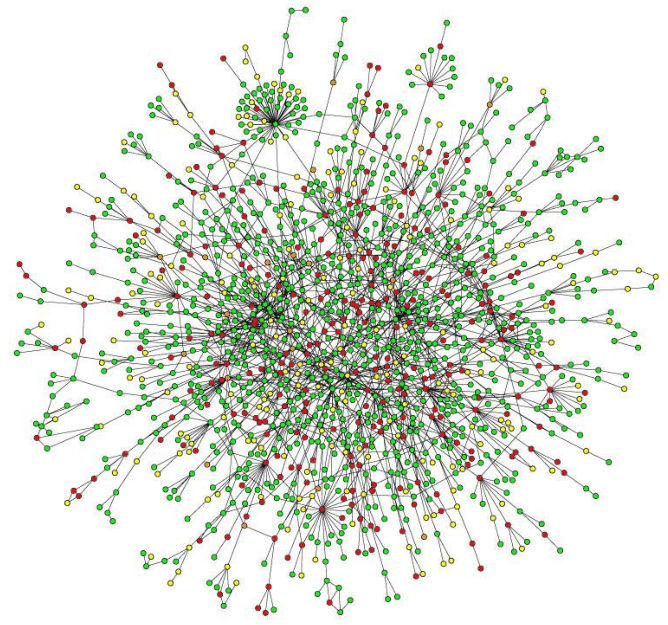
\includegraphics[scale=1.8]{scale-free-network}
  \caption{A Scale-Free Network (Yeast Proteome) \cite{wangKineticConformationalCharacterization}}
  \label{fig:scale-free}
\end{figure}


\subsection{Near-Reducibility}
Consider a Markov chain given by
$P=\begin{bsmallmatrix} 1 & 0 \\ 0 & 1 \end{bsmallmatrix}$. The chain is fully
reducible, and equivalently, the underlying graph is disconnected. Clearly, $P$
will only have eigenvalue 1 with multiplicity 2. Suppose now we have a chain
with
$P'=\begin{bsmallmatrix} 1 - \epsilon_1 & \epsilon_1 \\ \epsilon_2 & 1 -
  \epsilon_2 \end{bsmallmatrix}$, for $\epsilon \in (1,0)$. Thus, the spectrum
$\sigma(P') =P' \{ 1, 1-\epsilon_1 - \epsilon_2 \}$.

Nearly-reducible Markov chains have strong interactions within their clusters,
but relatively weak interactions between clusters.\footnote{The formal study of
  clustering in Markov chains is a well-developed field much more clearly
  understood through the probabilistic convergence theorem, which we have
  eschewed in this paper for a linear-algebraic focus. Powerful analysis of
  graph clustering and subdominant eigenvalues can also be done through the
  graph Laplacian, but we will not expound that tool here.} Considering the
canonical form of reducibility in Equation \eqref{eqn:reducible}, we note that
an irreducible Markov chain with subdominant eigenvalue $\lambda_2 \approx 1$
will be nearly reducible. However, the existence of such a subdominant
eigenvalue does not itself ensure near-reducibility.


\subsection{Scale-Free Networks}
In 1959, Erdős and Rényi proposed generating random graphs by considering a
Poisson distribution over the out-degree of vertices. In such a random graph
(also called an exponential network), most nodes share a similar number of
out-links, and there are very few nodes that deviate from this mean. A random
network is thus very democratic and has a steep bell curve. Most natural
networks, however, do not follow a random structure.
\begin{figure}
  \centering
  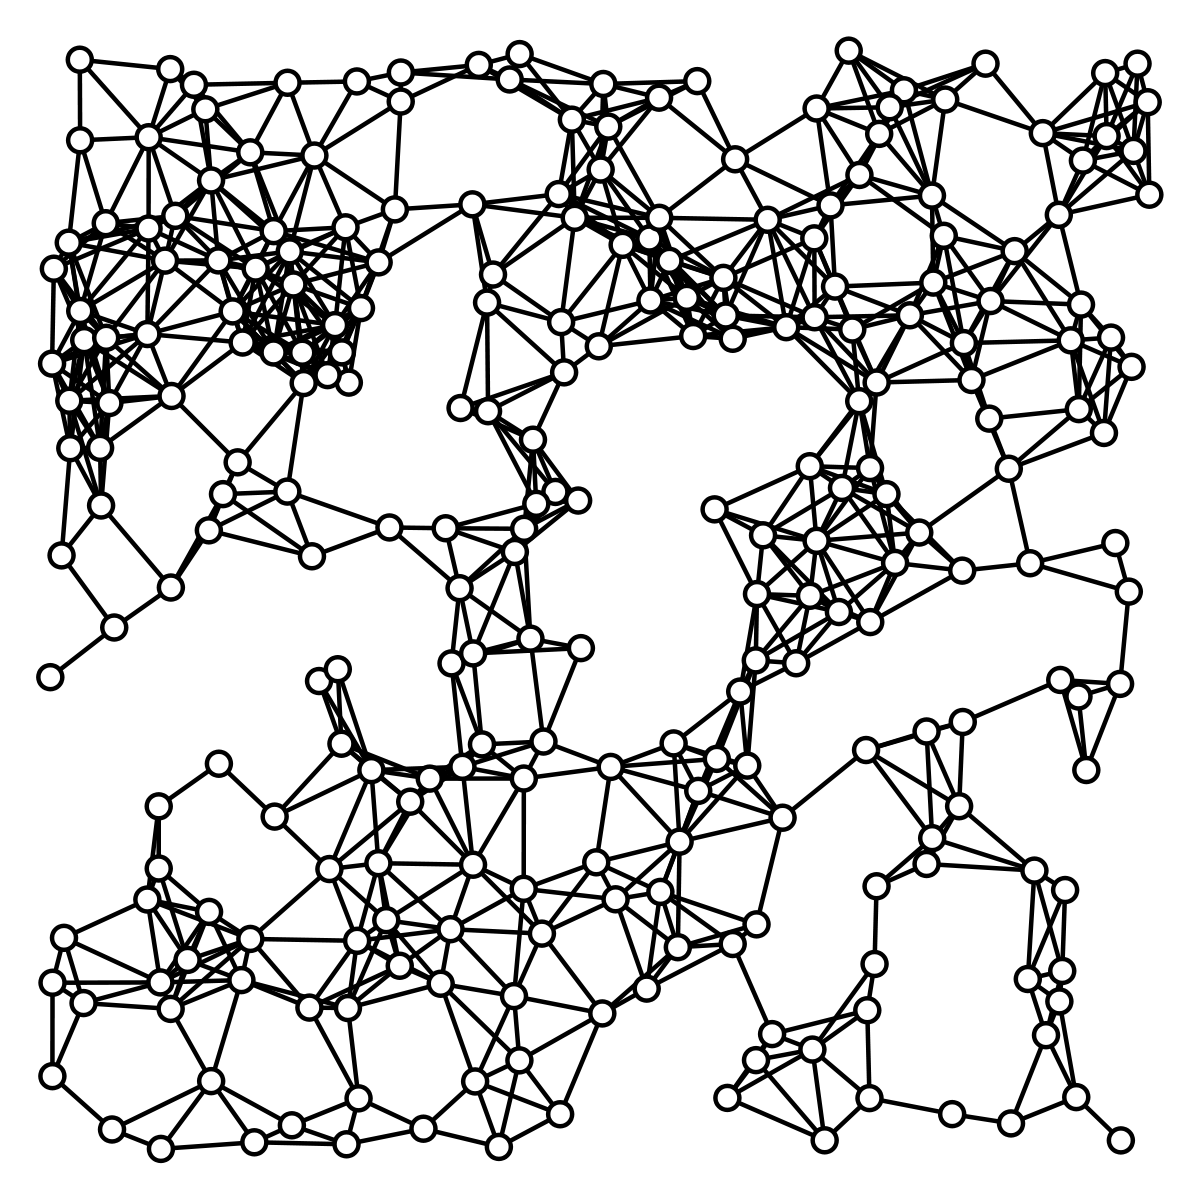
\includegraphics[scale=0.15]{random-graph}
  \caption{A Random Graph \cite{RandomGeometricGraph}}
  \label{fig:random}
\end{figure}
Consider Figure \ref{fig:scale-free}, which maps the partial proteome of a
yeast. The red nodes, which denote proteins most essential for life, tend to
bind together clusters of proteins of lesser importance. Note our use of the
term \textit{importance} here. If we only had the proteome graph, sans color, we
would likely be able to determine which proteins were most ``important'' for
life by computing a spectral rank like the PageRank. Indeed, we have assumed
from the start that the most connected nodes are the most important nodes. In
fact, HITS -- another spectral rank developed at IBM contemporaneously with
PageRank -- makes the pursuit more explicit by splitting Web pages into hubs and
authorities; it uses the more complex heuristic that good hubs link to good
authorities and vice versa. In a random graph, however, such a definition of
importance breaks down.

A music theorist analyzes a piece of classical music by first determining what
chords are most important -- that is, what chords are most tonally connected to
other chords. However, an atonal piece by Schönberg defies such straightforward
analysis. A twelve-tone series ensures an equal distribution of tones so no few
tones or chords distinguish themselves as tonally important, just as a random
graph ensures no few nodes stand out.\footnote{Note that this does not mean
  atonal music is ``random" in the standard sense; just like an Erdős-Rényi
  random graph, an atonal piece provides little information about the
  connections between tones. Thus, from a tonal perspective, we cannot easily
  determine which chords are more important than others. Tonality concerns
  itself about relations between chords, and these relations are evenly
  distributed by design in a twelve-tone piece. The progressions in such a piece
  mostly sound alike to our tonal ears, except for a few serendipitous ones that
  give a fleeting sense of tonality. This perhaps gives
  insight into why Schönberg abhored the label \textit{atonal} and much
  preferred to call his music \textit{pan-tonal}.}

Networks such as these follow a power law. The probability that a node has $k$
outlinks is proportional to $1/k^\gamma$, for some power $\gamma$. Although most
nodes have only a few links to others, a few have thousands. Removing just these
most important nodes (the hubs) can catastrophically fragment the network into
its isolated components disrupt the network. These networks also reveal a
beautiful fractal structure, so we we call them scale-free networks.
Sociologists have long known of these networks. The Erdős number and the ``six
degrees of Kevin Bacon'' work because a few people are highly connected; they
bridge groups of people who would otherwise be unrelated. Income distribution in
Western countries can be similarly modeled with a scale-free network. Note that
scale-free networks will also be very reducible, as they have strong
interactions within their clusters but relatively weak interactions among them.

Both the physical and logical Internet have been shown to be scale-free
networks. The Internet is thus highly resilient to random attacks, but
destroying just about 3\% of hubs -- the most highly connected ones -- would be
enough to fragment the Internet into dozens of isolated components
\cite{barabasiNetworkScienceScaleFree}. This suggests that even the large SCC of
Figure \ref{fig:web} is vulnerable to targeted attacks. By contrast, the
strongly-connected components of a random graph would be quite strong, as a
random graph does not encode much information in unique locations.

As we have seen, only scale-free networks have a sufficiently heterogeneous,
information-rich structure to permit a meaningful spectral importance rank.
Thus, Markov chains over scale-free networks will have a subdominant eigenvalue
quite close to $\lambda_1 = 1$. Although the teleportation adjustment ensured
the primitivity of the Google matrix, it still tends to leave the dampened Web
only weakly irreducible -- that is, nearly reducible.


\subsection{Damping Factor}
Recall $\alpha$, the damping factor used in Equation \eqref{eqn:google_matrix}.
This probability $\alpha$ controls the fidelity of the model to the raw Web
structure. As $\alpha \to 1$, the Google matrix becomes more nearly reducible,
its subdominant eigenvalue $\lambda \to 1$, and the power method converges ever
more slowly. Moreover, as $\alpha \to 1$, the limiting distribution becomes far
more sensitive -- both in terms of importance score and the consequent PageRanks
-- to link changes even within minor clusters; further approaching 1 magnifies
these effects. We can explore these results more by analyzing the vector
derivative $\dee\pi(\alpha)/\dee\alpha}$, but we will not do so here.

We learn in \cite{haveliwalaSecondEigenvalueGoogle} that a stochastic matrix $S$
with $\sigma_S = \{ 1, \lambda_2, \lambda_3, \cdots, \lambda_n \}$ gives a
Google matrix with
$\sigma_G = \alpha\sigma_S = \{ \alpha, \alpha\lambda_2, \alpha\lambda_3,
\cdots, \alpha\lambda_n \}$. From this, we see $\lambda_2 \leq \alpha$ for the
Google matrix. Thus, the power method converges at the rate which
$\alpha^k \to 0$ as $k$ grows. With $\alpha = 0.85$, Google's formulation of the
power method converges within a thousandth by approximately 50 iterations. Note
that the power method scales well to immense datasets like the Web graph -- it
requires at most 100 iterations to converge upon a unique ranking all pages on
the indexed Web.



\section{Evaluation}
Since PageRank incorporates the entire Web into its calculation, it is
query-independent. The refinements given in
\cite{haveliwalaAnalyticalComparisonApproaches2003} adapt the stochasticity and
teleportation distributions to provide a personalized PageRank. Query-dependent
algorithms like HITS beat PageRank in personalized searching, as they run a
power method on small components of the Web. However, the more serious induced
deficiencies -- like more imprecise ranking and susceptibility to link spamming
-- have made PageRank the dominant spectral ranking algorithm on the Web.
Moreover, the definition of importance built into PageRank means it can predict
backlinks (citations) well; Brin and Page \cite{brinPageRankCitationRanking1998}
showed that PageRank determines an optimal path for Web crawlers, who should
index the most important parts of the Web quickly and not be trapped by
closely-linked local chains.

Google still relies heavily upon the traditional vector space relevance models
and sophisticated analysis of anchor text, font style, and capitalization.
PageRank, after all, addresses a specific problem of structural relevance; other
systems must decide the a page's contextual relevance to a query. PageRank,
however, forms the central part of Google's search strategy -- a system designed
to scale even to a Web with $10^{100}$ pages -- a \textit{googol}.

\newpage
\bibliographystyle{ieeetr}
\bibliography{references}
\end{document}
